\appendix

\begin{figure*}
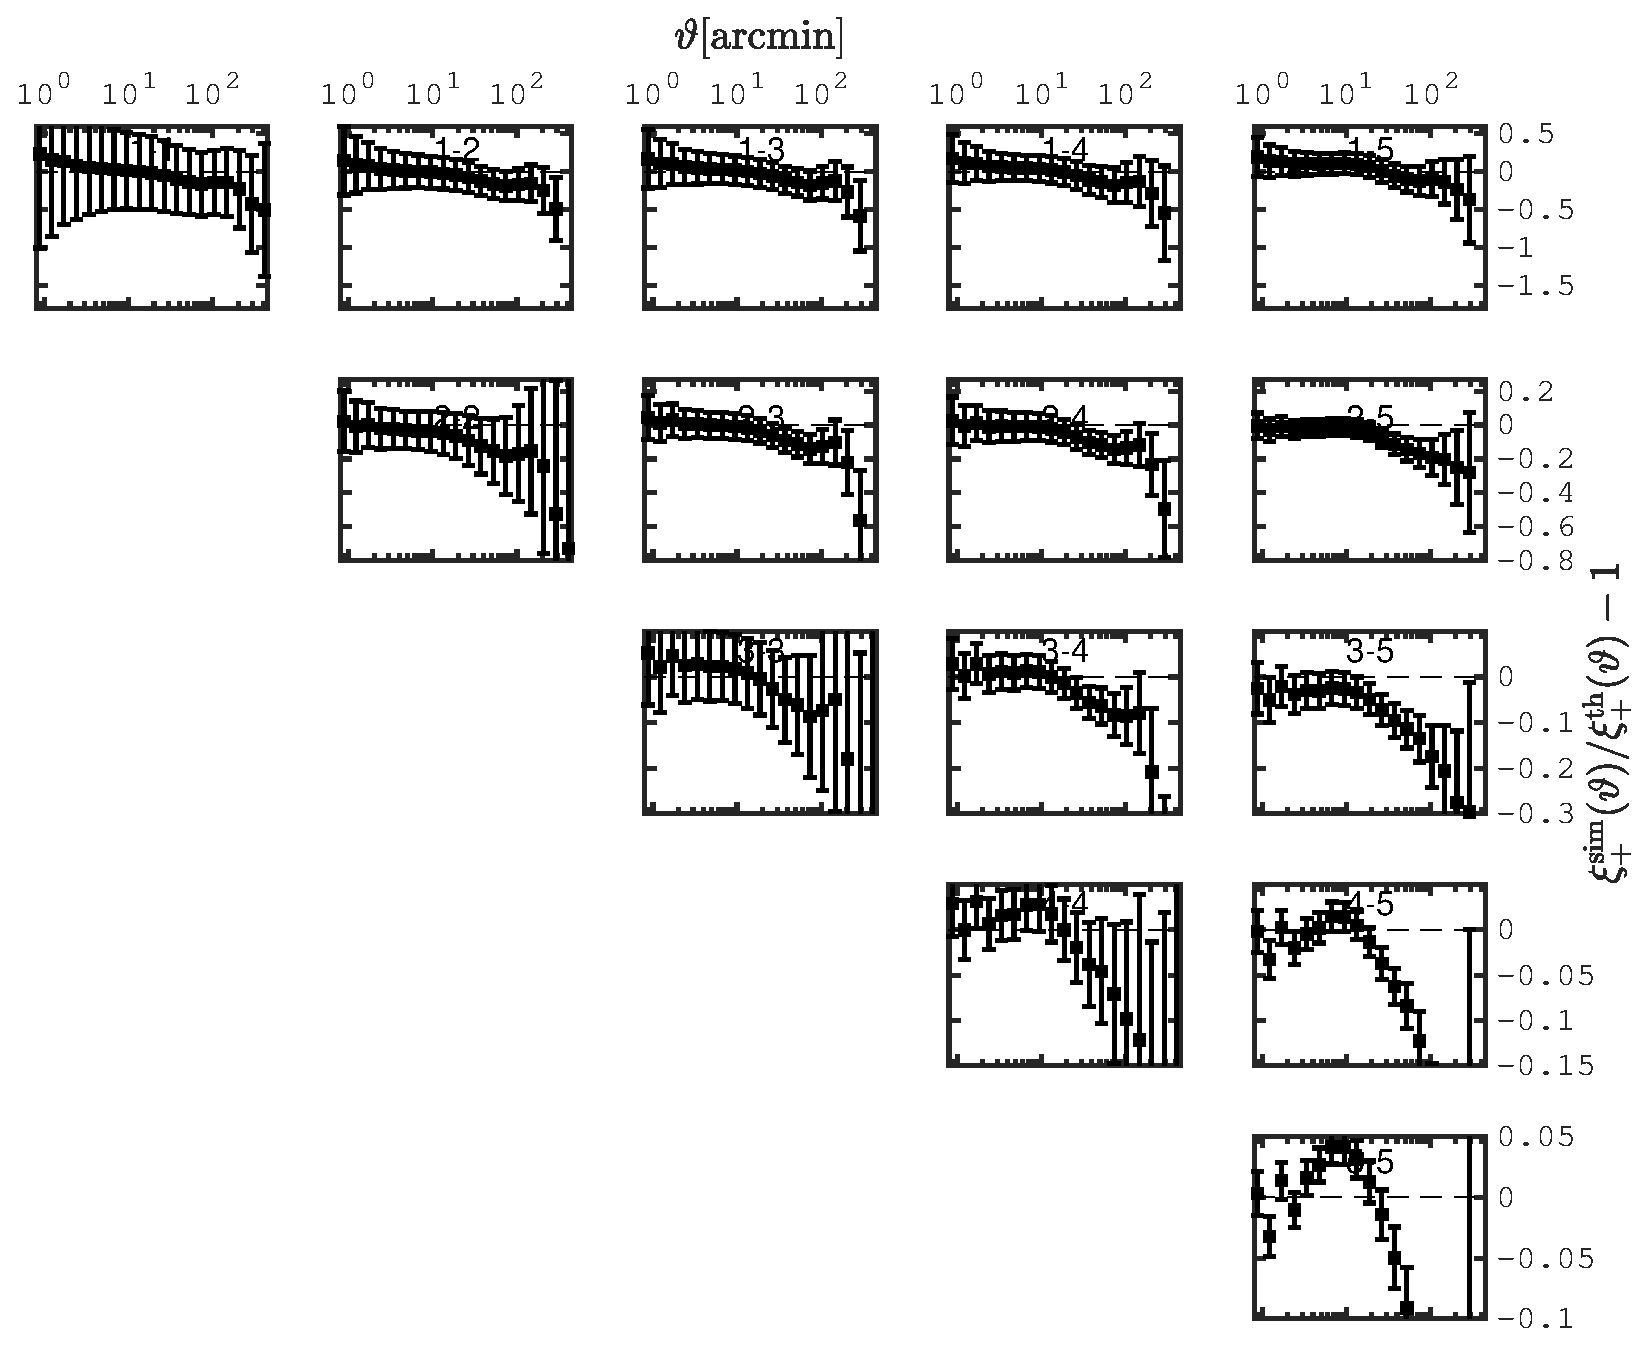
\includegraphics[width=\columnwidth]{graphs/xip_sims_vs_th.eps}
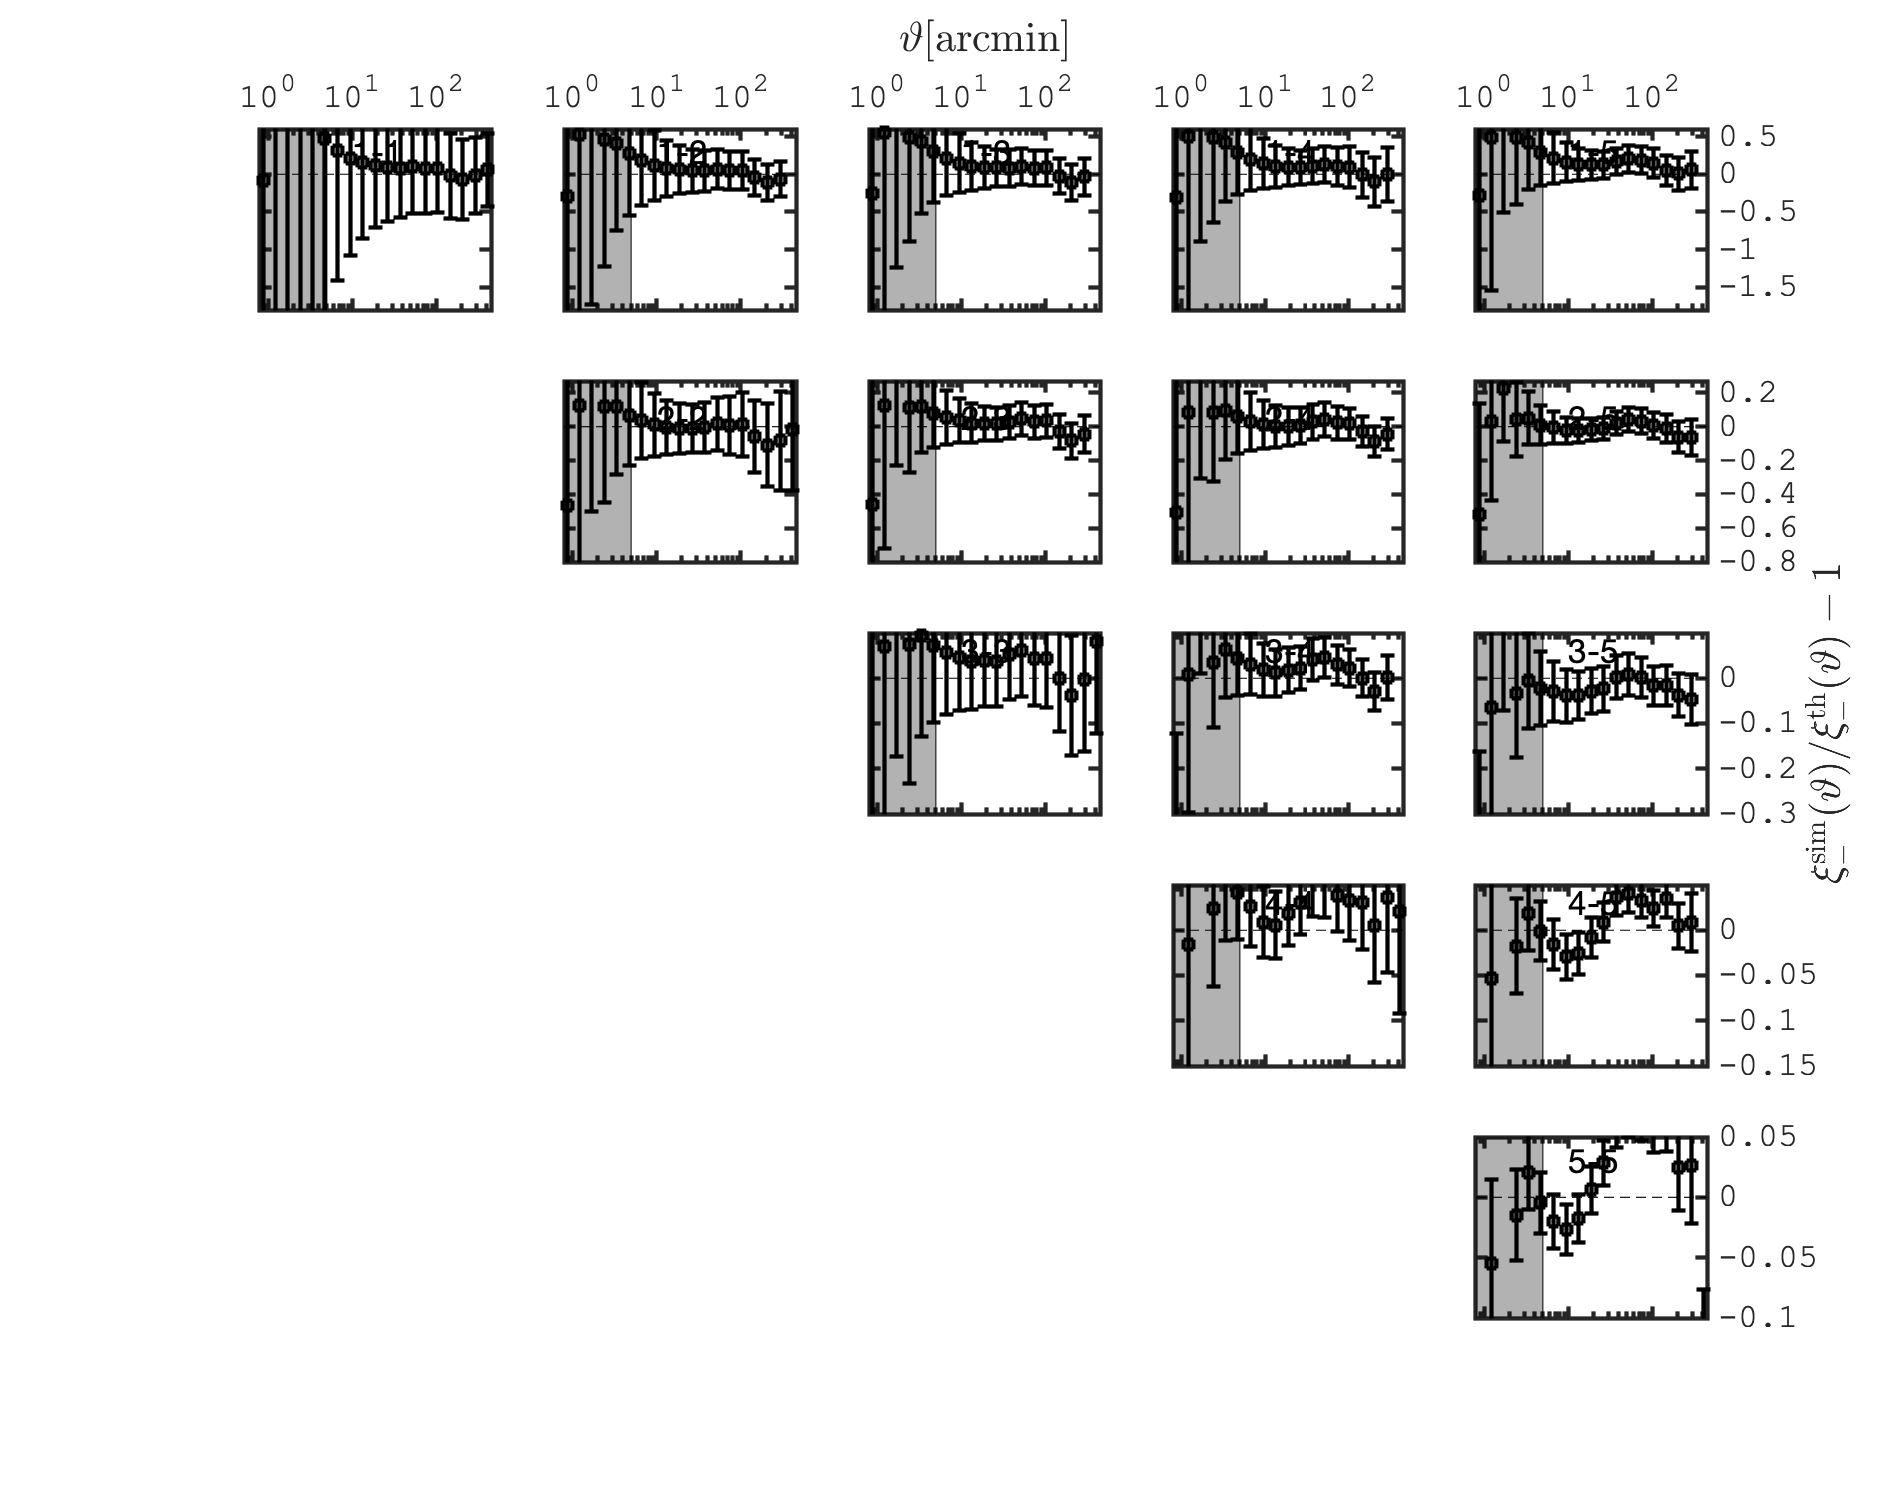
\includegraphics[width=\columnwidth]{graphs/xim_sims_vs_th.eps}
\caption{Fractional difference on $\xi_\pm$ between the measurements from SkySim5000 and the model predictions.  }
\label{fig:frac_err_sims_th}
\end{figure*}

\section{Projected Tidal Field}
\label{app:2d_TT}


\JHD{[To reword]} We derive in this Appendix...  
The prescription to assign an intrinsic alignment based on the projected tidal field, described in Eq. (\ref{eq:tidal_th}), involves the combinations $(s_{xx} - s_{yy})$ and $s_{xy}$, which therefore correspond to:
\begin{eqnarray}
 \widetilde{\epsilon}_1^{\rm IA} (\boldsymbol k_{\perp})  &\propto& \left(\frac{k_x^2 - k_y^2}{k^2} \right) \widetilde{\delta}_{\rm 2D}(\boldsymbol k_{\perp})\mathcal{G_{\rm 2D}}(\sigma_{\rm G})  \, ,\nonumber \\
 \widetilde{\epsilon}_2^{\rm IA} (\boldsymbol k_\perp)  &\propto& \left(\frac{k_x k_y}{k^2} \right) \widetilde {\delta}_{\rm 2D}(\boldsymbol k_\perp)\mathcal{G_{\rm 2D}}(\sigma_{\rm G}) 
 %\label{eq:sij}
\end{eqnarray}

Aside from the smoothing kernel, these are the same filters that are used for converting convergence maps to shear maps under the \citet[][KS hereafter]{KaiserSquires} inversion:
 \begin{eqnarray}
 \widetilde{\gamma_1} (\boldsymbol \ell)  = \left(\frac{k_x^2 - k_y^2}{k^2} \right) \widetilde {\kappa}(\boldsymbol \ell) \, , \hspace{1cm} \widetilde{\gamma_2} (\boldsymbol \ell)  = \left(\frac{k_x k_y}{k^2} \right) \widetilde {\kappa}(\boldsymbol \ell)
 %\label{eq:sij}
\end{eqnarray}
meaning that on can linearly combine the mass sheets with the correct coefficients and obtain intrinsic ellipticities from a normal KS inversion. 

Projecting out the $z$ components (e.i. $s_{0i}$=$s_{i0}$=0 for all $i$),  the tidal torque terms from Eq. (\ref{eq:tidal_th_TT}) can be expanded as:
 \begin{eqnarray}
\gamma^{\rm TT}_{ij}&=& C_2 \left[\sum_{k=x,y} s_{ik} s_{kj} -\frac{1}{3} \delta_{ij} s^2\right] \\
                                  &=&C_2 \left[ s_{ix}s_{xj}  + s_{iy}s_{yj}  -  \frac{1}{3} \delta_{ij} \left( s_{xx}^2 + s_{yy}^2 +2s_{xy}^2 \right)  \right] \, .
\end{eqnarray}
Specifically, this yields:
 \begin{eqnarray}
\gamma^{\rm TT}_{xx}&=& C_2 \left[\frac{2}{3}s_{xx}^2  -  \frac{1}{3}s_{yy}^2 + \frac{1}{3}s_{xy}^2 \right]\, ,  \nonumber \\
\gamma^{\rm TT}_{yy}&=& C_2 \left[-\frac{1}{3}s_{xx}^2  +  \frac{2}{3}s_{yy}^2 + \frac{1}{3}s_{xy}^2  \right]\, , \\
\gamma^{\rm TT}_{xy}&=& C_2 s_{xy}\left[s_{xx}+s_{yy}  \right]\, . \nonumber                                  
\end{eqnarray}
With the standard ellipticity definitions $\epsilon_1^{\rm TT}\equiv \gamma_{xx}^{\rm TT} - \gamma_{yy}^{\rm TT}$ and $\epsilon_2^{\rm TT}\equiv -2 \gamma_{xy}$, we obtain:
\begin{eqnarray}
\epsilon_1^{\rm TT} = C_2  \left[ s_{xx}^2 - s_{yy}^2\right] \, , \epsilon_2^{\rm TT} = -2 C_2 s_{xy}\left[s_{xx}+s_{yy}  \right]\, .
\end{eqnarray}
In the TATT model, the total intrinsic ellipticity component is therefore given by $\epsilon_{1/2}^{\rm IA} = \epsilon_{1/2}^{\rm TATT} = \epsilon_{1/2}^{\delta{\rm-NLA}} + \epsilon_{1/2}^{\rm TT}$.